\usetikzlibrary{automata,arrows}


Als erstes müssen wir den DFA A in A$rev$, also den DFA der all jene Eingaben akzeptiert die das Teilwort $deer$ enthalten.

Hierfür werden alle Kanten umgedreht und Start- und Endzustand vertauscht.

So wird

\begin{figure}[ht]
\centering
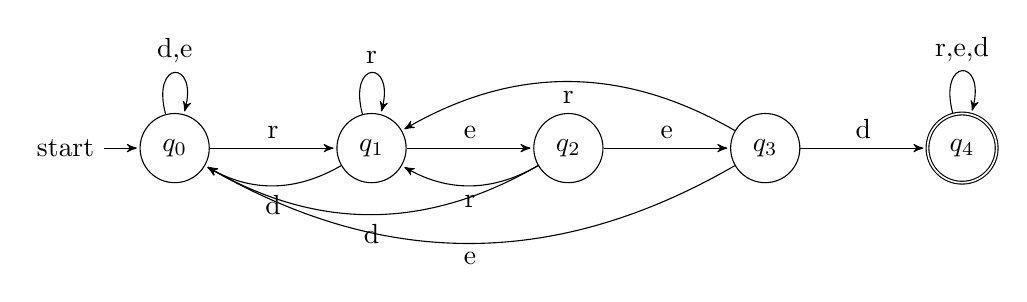
\begin{tikzpicture}[->,>=stealth',shorten >=1pt,auto,node distance=2.5 cm, scale = 1, transform shape]

%\tikzstyle{every state}=[fill=white,draw=black,text=black]

%Erstelle 5 Zustände

\node[initial,state]	(A)					{$q_0$};
\node[state]			(B)	[right of =A]	{$q_1$};
\node[state]			(C)	[right of =B]	{$q_2$};
\node[state]			(D)	[right of =C]	{$q_3$};
\node[state,accepting]	(E)	[right of =D]	{$q_4$};

%Erstelle Übergänge
\path	(A)	edge					node	{r} 	(B)
			edge	[loop above]	node	{d,e}	(A)
		(B)	edge					node	{e}		(C)
			edge	[loop above]	node	{r}		(B)
			edge	[bend left]		node	{d}		(A)
		(C) edge					node	{e}		(D)
			edge	[bend left]		node	{r}		(B)
			edge	[bend left]		node	{d}		(A)
		(D) edge					node	{d}		(E)
			edge	[bend right]	node	{r}		(B)
			edge	[bend left]		node	{e}		(A)
		(E) edge	[loop above]	node	{r,e,d}	(E);


\end{tikzpicture}
\caption{Der Ursprüngliche DFA A}
\end{figure}

in 

\begin{figure}[ht]
\centering
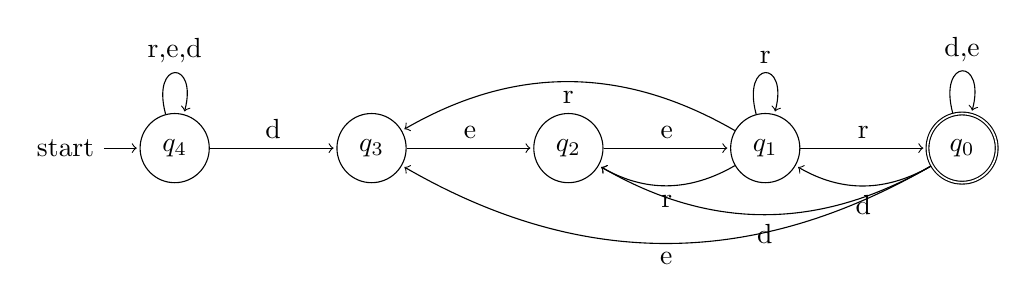
\begin{tikzpicture}[->,shorten >=1pt,auto,node distance=2.5 cm, scale = 1, transform shape]

%\tikzstyle{every state}=[fill=white,draw=black,text=black]

%Erstelle 5 Zustände

\node[state,initial]	(E)					{$q_4$};
\node[state]			(D)	[right of =E]	{$q_3$};
\node[state]			(C)	[right of =D]	{$q_2$};
\node[state]			(B)	[right of =C]	{$q_1$};
\node[state,accepting]	(A)	[right of =B]	{$q_0$};

%Erstelle Übergänge
\path	(A)	edge	[loop above]	node	{d,e}	(A)
			edge	[bend left]		node	{d}		(B)
			edge	[bend left]		node	{d}		(C)
			edge	[bend left]		node	{e}		(D)
		(B)	edge					node	{r}		(A)
			edge	[loop above]	node	{r}		(B)
			edge	[bend right]	node	{r}		(D)
			edge	[bend left]		node	{r}		(C)
		(C) edge					node	{e}		(B)
		(D) edge					node	{e}		(C)
		(E) edge					node	{d}		(D)
			edge	[loop above]	node	{r,e,d} (E);

\end{tikzpicture}
\caption{Der NFA A rev}
\end{figure}

umgewandelt.

Anschließend benutzen wir die Potenzautomatenkonstruktion um den Automaten in folgenden zu überführen:

\begin{figure}[ht]
\centering
\begin{tikzpicture}[->,shorten >=1pt,auto,node distance=2.5 cm, scale = 1, transform shape]

%\tikzstyle{every state}=[fill=white,draw=black,text=black]

%Erstelle 5 Zustände

\node[state,initial]	(E)			{$\{q_4\}$};
\node[state]		(ED)	[right of =E]	{$\{q_4,q_3\}$};
\node[state]		(C)	[right of =D]	{$\{q_2\}$};
\node[state]		(B)	[right of =C]	{$\{q_1\}$};
\node[state,accepting]	(A)	[right of =B]	{$\{q_0\}$};
\node[state,accepting]	(ABCD)	[above of =B]	{$\{q_0,q_1,q_2,q_3\}$};



%Erstelle Übergänge
\path	(E) 	edge	[loop above]	node 	{r,e}	(E)
		edge	[bend left]	node	{d}		(ED)
	(ED)	edge	[bend left]	node	{e}		(C)
		edge	[bend left]	node	{r}		(E)
		edge	[loop below]	node	{d}	(D)
	(C)	edge	[bend left]	node	{r,d}	(ED)
		edge			node	{e}		(B)
	(B)	edge	[bend left]	node	{e,d}	(B)
		edge	[bend right]	node	{r}		(ABCD);
\end{tikzpicture}
\caption{Der Potenzautomat A rev}
\end{figure}


Damit haben wir den Algorithmus abgearbeitet und einen Automaten erzeugt der das gewünschte leistet (wie in 5. gezeigt wird).